\documentclass{standalone}
\usepackage{tikz}
\usetikzlibrary{patterns, positioning}


\begin{document}
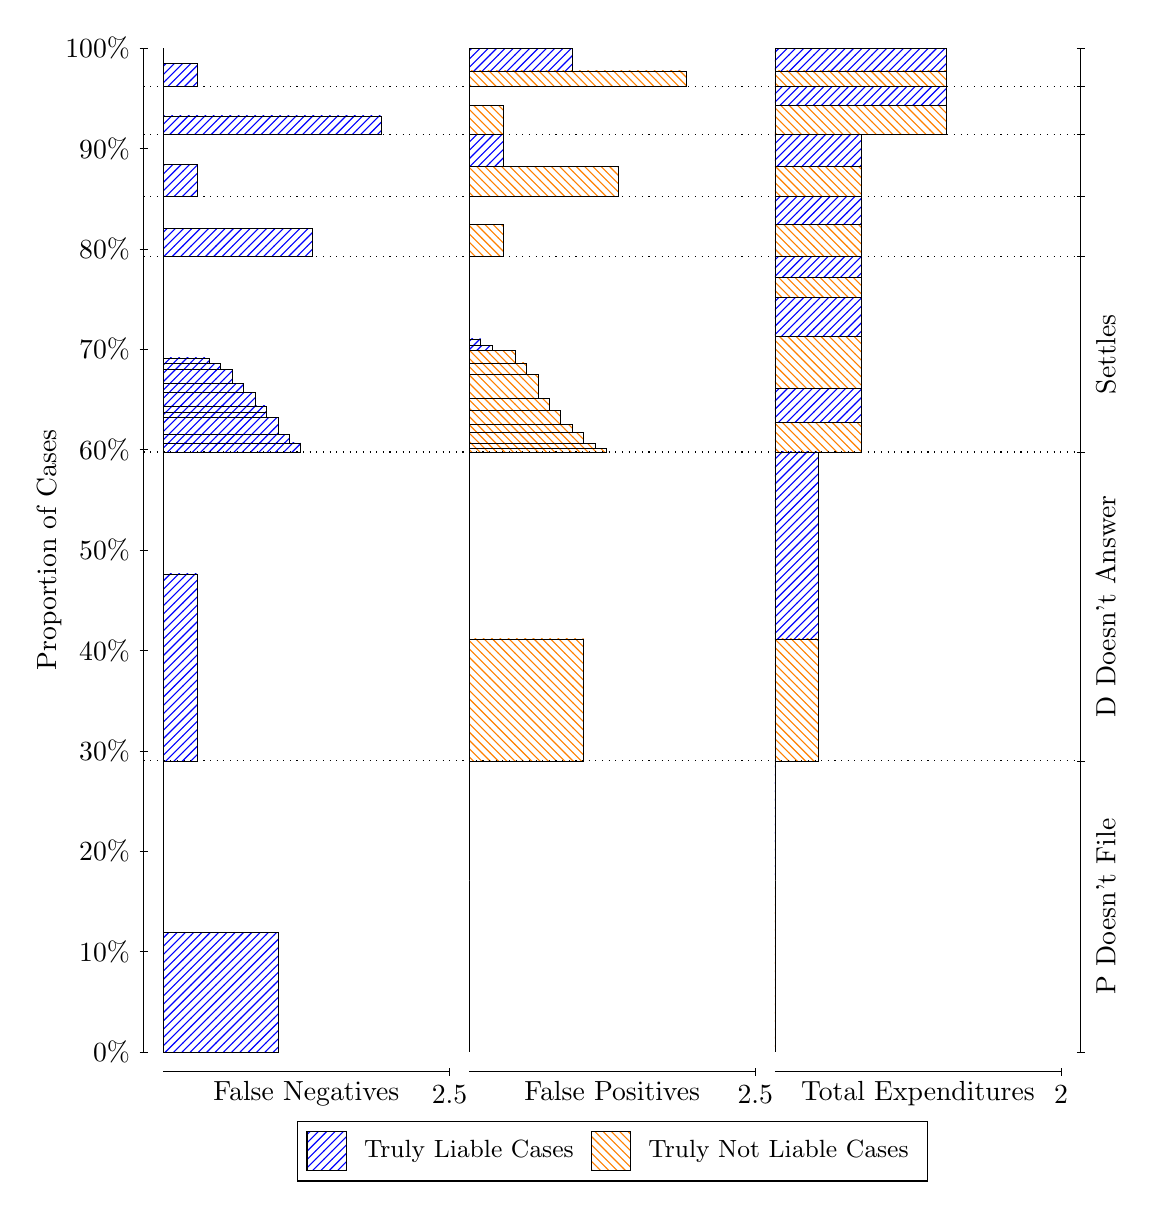
\begin{tikzpicture}
\draw[black, very thin] (1.5,1.75) -- (1.5,14.5);
\node[rotate=90, text=black, anchor=center] at (0.3, 8.125) {Proportion of Cases};
\draw[black, very thin] (1.45,1.75) -- (1.55,1.75);
\node[text=black, anchor=east] at (1.45, 1.75) {0\%};
\draw[black, very thin] (1.45,3.025) -- (1.55,3.025);
\node[text=black, anchor=east] at (1.45, 3.025) {10\%};
\draw[black, very thin] (1.45,4.3) -- (1.55,4.3);
\node[text=black, anchor=east] at (1.45, 4.3) {20\%};
\draw[black, very thin] (1.45,5.575) -- (1.55,5.575);
\node[text=black, anchor=east] at (1.45, 5.575) {30\%};
\draw[black, very thin] (1.45,6.85) -- (1.55,6.85);
\node[text=black, anchor=east] at (1.45, 6.85) {40\%};
\draw[black, very thin] (1.45,8.125) -- (1.55,8.125);
\node[text=black, anchor=east] at (1.45, 8.125) {50\%};
\draw[black, very thin] (1.45,9.4) -- (1.55,9.4);
\node[text=black, anchor=east] at (1.45, 9.4) {60\%};
\draw[black, very thin] (1.45,10.675) -- (1.55,10.675);
\node[text=black, anchor=east] at (1.45, 10.675) {70\%};
\draw[black, very thin] (1.45,11.95) -- (1.55,11.95);
\node[text=black, anchor=east] at (1.45, 11.95) {80\%};
\draw[black, very thin] (1.45,13.225) -- (1.55,13.225);
\node[text=black, anchor=east] at (1.45, 13.225) {90\%};
\draw[black, very thin] (1.45,14.5) -- (1.55,14.5);
\node[text=black, anchor=east] at (1.45, 14.5) {100\%};

\draw[black, very thin] (13.4,1.75) -- (13.4,14.5);
\draw[black, very thin] (13.35,1.75) -- (13.45,1.75);
\node[anchor=west] at (13.35, 1.75) {};
\draw[black, very thin] (13.35,5.4475) -- (13.45,5.4475);
\node[anchor=west] at (13.35, 5.4475) {};
\draw[black, very thin] (13.35,9.3703) -- (13.45,9.3703);
\node[anchor=west] at (13.35, 9.3703) {};
\draw[black, very thin] (13.35,11.852) -- (13.45,11.852);
\node[anchor=west] at (13.35, 11.852) {};
\draw[black, very thin] (13.35,12.618) -- (13.45,12.618);
\node[anchor=west] at (13.35, 12.618) {};
\draw[black, very thin] (13.35,13.4) -- (13.45,13.4);
\node[anchor=west] at (13.35, 13.4) {};
\draw[black, very thin] (13.35,14.012) -- (13.45,14.012);
\node[anchor=west] at (13.35, 14.012) {};
\draw[black, very thin] (13.35,14.5) -- (13.45,14.5);
\node[anchor=west] at (13.35, 14.5) {};

\draw[black, very thin, pattern color=blue, pattern=north east lines] (1.75,1.75) rectangle (3.2033,3.2701);
\draw[black, very thin, pattern color=orange, pattern=north west lines] (1.75,3.2701) rectangle (1.75,5.4475);
\draw[black, very thin, pattern color=blue, pattern=north east lines] (1.75,5.4475) rectangle (2.186,7.8216);
\draw[black, very thin, pattern color=orange, pattern=north west lines] (1.75,7.8216) rectangle (1.75,9.3703);
\draw[black, very thin, pattern color=blue, pattern=north east lines] (1.75,9.3703) rectangle (3.494,9.4857);
\draw[black, very thin, pattern color=blue, pattern=north east lines] (1.75,9.4857) rectangle (3.3487,9.5948);
\draw[black, very thin, pattern color=blue, pattern=north east lines] (1.75,9.5948) rectangle (3.2033,9.8137);
\draw[black, very thin, pattern color=blue, pattern=north east lines] (1.75,9.8137) rectangle (3.058,9.8742);
\draw[black, very thin, pattern color=blue, pattern=north east lines] (1.75,9.8742) rectangle (3.058,9.954);
\draw[black, very thin, pattern color=blue, pattern=north east lines] (1.75,9.954) rectangle (2.9127,10.126);
\draw[black, very thin, pattern color=blue, pattern=north east lines] (1.75,10.126) rectangle (2.7673,10.238);
\draw[black, very thin, pattern color=blue, pattern=north east lines] (1.75,10.238) rectangle (2.622,10.417);
\draw[black, very thin, pattern color=blue, pattern=north east lines] (1.75,10.417) rectangle (2.4767,10.496);
\draw[black, very thin, pattern color=blue, pattern=north east lines] (1.75,10.496) rectangle (2.3313,10.564);
\draw[black, very thin, pattern color=orange, pattern=north west lines] (1.75,10.564) rectangle (1.75,11.852);
\draw[black, very thin, pattern color=blue, pattern=north east lines] (1.75,11.852) rectangle (3.6393,12.207);
\draw[black, very thin, pattern color=orange, pattern=north west lines] (1.75,12.207) rectangle (1.75,12.618);
\draw[black, very thin, pattern color=blue, pattern=north east lines] (1.75,12.618) rectangle (2.186,13.023);
\draw[black, very thin, pattern color=orange, pattern=north west lines] (1.75,13.023) rectangle (1.75,13.4);
\draw[black, very thin, pattern color=blue, pattern=north east lines] (1.75,13.4) rectangle (4.5113,13.637);
\draw[black, very thin, pattern color=orange, pattern=north west lines] (1.75,13.637) rectangle (1.75,14.012);
\draw[black, very thin, pattern color=blue, pattern=north east lines] (1.75,14.012) rectangle (2.186,14.301);
\draw[black, very thin, pattern color=orange, pattern=north west lines] (1.75,14.301) rectangle (1.75,14.5);
\draw[black, very thin, pattern color=orange, pattern=north west lines] (5.6333,1.75) rectangle (5.6333,3.9274);
\draw[black, very thin, pattern color=blue, pattern=north east lines] (5.6333,3.9274) rectangle (5.6333,5.4475);
\draw[black, very thin, pattern color=orange, pattern=north west lines] (5.6333,5.4475) rectangle (7.0867,6.9963);
\draw[black, very thin, pattern color=blue, pattern=north east lines] (5.6333,6.9963) rectangle (5.6333,9.3703);
\draw[black, very thin, pattern color=orange, pattern=north west lines] (5.6333,9.3703) rectangle (7.3773,9.4194);
\draw[black, very thin, pattern color=orange, pattern=north west lines] (5.6333,9.4194) rectangle (7.232,9.4802);
\draw[black, very thin, pattern color=orange, pattern=north west lines] (5.6333,9.4802) rectangle (7.0867,9.6152);
\draw[black, very thin, pattern color=orange, pattern=north west lines] (5.6333,9.6152) rectangle (6.9413,9.7243);
\draw[black, very thin, pattern color=orange, pattern=north west lines] (5.6333,9.7243) rectangle (6.796,9.9003);
\draw[black, very thin, pattern color=orange, pattern=north west lines] (5.6333,9.9003) rectangle (6.6507,10.054);
\draw[black, very thin, pattern color=orange, pattern=north west lines] (5.6333,10.054) rectangle (6.5053,10.354);
\draw[black, very thin, pattern color=orange, pattern=north west lines] (5.6333,10.354) rectangle (6.36,10.501);
\draw[black, very thin, pattern color=orange, pattern=north west lines] (5.6333,10.501) rectangle (6.2147,10.658);
\draw[black, very thin, pattern color=blue, pattern=north east lines] (5.6333,10.658) rectangle (5.924,10.726);
\draw[black, very thin, pattern color=blue, pattern=north east lines] (5.6333,10.726) rectangle (5.7787,10.805);
\draw[black, very thin, pattern color=blue, pattern=north east lines] (5.6333,10.805) rectangle (5.6333,11.852);
\draw[black, very thin, pattern color=orange, pattern=north west lines] (5.6333,11.852) rectangle (6.0693,12.264);
\draw[black, very thin, pattern color=blue, pattern=north east lines] (5.6333,12.264) rectangle (5.6333,12.618);
\draw[black, very thin, pattern color=orange, pattern=north west lines] (5.6333,12.618) rectangle (7.5227,12.995);
\draw[black, very thin, pattern color=blue, pattern=north east lines] (5.6333,12.995) rectangle (6.0693,13.4);
\draw[black, very thin, pattern color=orange, pattern=north west lines] (5.6333,13.4) rectangle (6.0693,13.774);
\draw[black, very thin, pattern color=blue, pattern=north east lines] (5.6333,13.774) rectangle (5.6333,14.012);
\draw[black, very thin, pattern color=orange, pattern=north west lines] (5.6333,14.012) rectangle (8.3947,14.21);
\draw[black, very thin, pattern color=blue, pattern=north east lines] (5.6333,14.21) rectangle (6.9413,14.5);
\draw[black, very thin, pattern color=orange, pattern=north west lines] (9.5167,1.75) rectangle (9.5167,3.9274);
\draw[black, very thin, pattern color=blue, pattern=north east lines] (9.5167,3.9274) rectangle (9.5167,5.4475);
\draw[black, very thin, pattern color=orange, pattern=north west lines] (9.5167,5.4475) rectangle (10.062,6.9963);
\draw[black, very thin, pattern color=blue, pattern=north east lines] (9.5167,6.9963) rectangle (10.062,9.3703);
\draw[black, very thin, pattern color=orange, pattern=north west lines] (9.5167,9.3703) rectangle (10.607,9.7421);
\draw[black, very thin, pattern color=blue, pattern=north east lines] (9.5167,9.7421) rectangle (10.607,10.173);
\draw[black, very thin, pattern color=orange, pattern=north west lines] (9.5167,10.173) rectangle (10.607,10.835);
\draw[black, very thin, pattern color=blue, pattern=north east lines] (9.5167,10.835) rectangle (10.607,11.338);
\draw[black, very thin, pattern color=orange, pattern=north west lines] (9.5167,11.338) rectangle (10.607,11.592);
\draw[black, very thin, pattern color=blue, pattern=north east lines] (9.5167,11.592) rectangle (10.607,11.852);
\draw[black, very thin, pattern color=orange, pattern=north west lines] (9.5167,11.852) rectangle (10.607,12.264);
\draw[black, very thin, pattern color=blue, pattern=north east lines] (9.5167,12.264) rectangle (10.607,12.618);
\draw[black, very thin, pattern color=orange, pattern=north west lines] (9.5167,12.618) rectangle (10.607,12.995);
\draw[black, very thin, pattern color=blue, pattern=north east lines] (9.5167,12.995) rectangle (10.607,13.4);
\draw[black, very thin, pattern color=orange, pattern=north west lines] (9.5167,13.4) rectangle (11.697,13.774);
\draw[black, very thin, pattern color=blue, pattern=north east lines] (9.5167,13.774) rectangle (11.697,14.012);
\draw[black, very thin, pattern color=orange, pattern=north west lines] (9.5167,14.012) rectangle (11.697,14.21);
\draw[black, very thin, pattern color=blue, pattern=north east lines] (9.5167,14.21) rectangle (11.697,14.5);
\draw[black, dotted] (1.5,5.4475) -- (13.4,5.4475);
\draw[black, dotted] (1.5,9.3703) -- (13.4,9.3703);
\draw[black, dotted] (1.5,11.852) -- (13.4,11.852);
\draw[black, dotted] (1.5,12.618) -- (13.4,12.618);
\draw[black, dotted] (1.5,13.4) -- (13.4,13.4);
\draw[black, dotted] (1.5,14.012) -- (13.4,14.012);
\draw[black, very thin] (1.75,1.5) -- (5.3833,1.5);
\node[text=black, anchor=north] at (3.5667, 1.5) {False Negatives};
\draw[black, very thin] (5.3833,1.45) -- (5.3833,1.55);
\node[text=black, anchor=north] at (5.3833, 1.45) {2.5};

\draw[black, very thin] (5.6333,1.5) -- (9.2667,1.5);
\node[text=black, anchor=north] at (7.45, 1.5) {False Positives};
\draw[black, very thin] (9.2667,1.45) -- (9.2667,1.55);
\node[text=black, anchor=north] at (9.2667, 1.45) {2.5};

\draw[black, very thin] (9.5167,1.5) -- (13.15,1.5);
\node[text=black, anchor=north] at (11.333, 1.5) {Total Expenditures};
\draw[black, very thin] (13.15,1.45) -- (13.15,1.55);
\node[text=black, anchor=north] at (13.15, 1.45) {2};

\node[text=black, centered, rotate=90] at (13.72, 3.5988) {P Doesn't File};
\node[text=black, centered, rotate=90] at (13.72, 7.4089) {D Doesn't Answer};
\node[text=black, centered, rotate=90] at (13.72, 10.611) {Settles};





\draw (7.449999999999999,1.5) node[draw=none] (baseCoordinate) {};
\begin{scope}[align=center]
        \matrix[scale=0.5, draw=black, below=0.5cm of baseCoordinate, nodes={draw}, column sep=0.1cm]{
            \node[rectangle, draw, minimum width=0.5cm, minimum height=0.5cm, pattern color=blue, pattern=north east lines] {}; &
            \node[draw=none, font=\small, text=black] (B) {Truly Liable Cases}; &
            \node[rectangle, draw, minimum width=0.5cm, minimum height=0.5cm, pattern color=orange, pattern=north west lines] {}; &
            \node[draw=none, font=\small, text=black] (B) {Truly Not Liable Cases}; \\
            };
\end{scope}

\end{tikzpicture}
\end{document}